\section{Large Scale Terrain Generation from Tectonic Uplift and Fluvial Erosion}
At large scale, terrains and mountains are formed by various mutually interacting physical processes acting at geological time and spatial scales. The terrains we observe in nature result from the erosional response to tectonically-driven uplift. This paper\cite{cordonnier2016large} studies the role of the interaction between the uplift and the erosion caused by waterflow. The procedure generates large mountainous terrains with plausible large scale landform features and patterns. Rivers strongly form the appearance of terrains, therefore it is only plausible to include them in this simulation.
The user supplies an uplift map, a grey-scale map defining the speed at which the terrain is elevated by tectonics. From this input, a random planar graph is created. The method iterates over time steps the update the elevation of the graph and its surrounding environment. This method yields terrains that have a high grade of visual realism as shown in figure \ref{fig:visual_realism}

\begin{figure}[htb]	
	\centering
	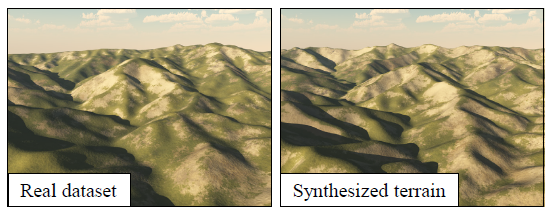
\includegraphics[width=\linewidth]{cordonnier2016large/visual_realism}
	\caption{Comparison of a real terrain and a model created by fluvial erosion simulation}
	\label{fig:visual_realism}
\end{figure}

\subsection{Algorithm Overview}
Over the domain of the uplift map the method generates a planar graph, describing a future network of rivers. Each node of the graph has a position and, more importantly, an elevation. 

Within this graph a set of stream trees is generated. The properties of such a stream tree will be described below. As the terrain is elevated, it is possible that lakes, that were formed earlier, overflow and therefore create new connections. The graph has to be modified to account for such changes each simulation step. 

Once the new connections are created the slope and drainage area of each node can be computed. This parameter heavily influences appearance of the river and the surrounding terrain. With this parameters, the stream power equation\cite{JGRB:JGRB11856} is solved to calculate the updated elevation of the graphs nodes. The now updated graph works as input for the next iteration step in this simulation. 
\ref{fig:stream_power_resolution_algorithm} shows an overview over the complete algorithm. 

\begin{figure}[htb]	
	\centering
	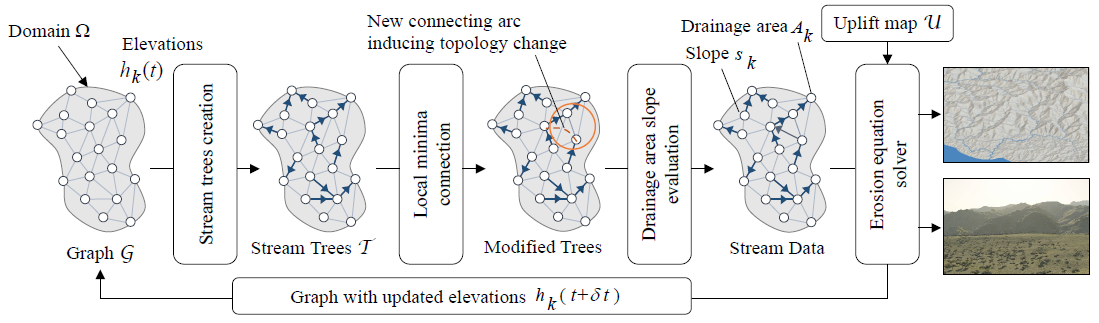
\includegraphics[width=\linewidth]{cordonnier2016large/stream_power_resolution_algorithm}
	\caption{Overview of the stream power resolution algorithm}
	\label{fig:stream_power_resolution_algorithm}
\end{figure}

\subsection{Stream Trees}
A stream tree is a directed subgraph of the graph which follows the principles of a river. Water only flows downwards, therefore the direction of node connections are towards the node with the lower elevation. Nodes that can not be connect further to a tree describe a local minimum and therefore a lake will form on this node. 

\subsection{Stream Power Equation}
The stream power equation describes the interaction between the fluvial erosion and the tectonic uplift. It takes into account the slope of the terrain, the position, as well the drainage area. This equation solved will yield in an updated elevation that takes fluvial erosion and uplift into account. 

\subsection{Iterative Growth of Terrain}
As mentioned above, the procedure iteratively is repeated in order to simulate a continious tectonic uplift. Whilst the method itself delivers fairly good looking results, the procedure lives from iterative growth of the graph. This way the terrain forming over geological time steps can be simulated. Figure \ref{fig:iterations} shows the iterative growth of a terrain. To give a better insight of the scales of the simulation, in this example the algorithm uses timestep of $2.500 \cdot 10^5$ years and a tectonic uplift rate of $5.0 \cdot 10^{-4}$ meters. This translates to a maximum change in elevation each time step of 125 meters. 

\begin{figure}[htb]	
	\centering
	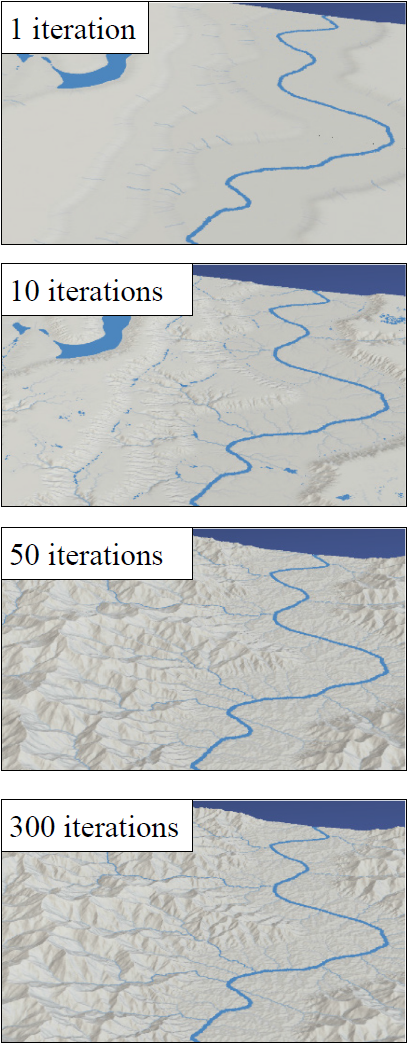
\includegraphics[width=0.8\linewidth]{cordonnier2016large/iterations}
	\caption{Growth of the terrain after different timesteps of the simulation.}
	\label{fig:iterations}
\end{figure}

\subsection{Representation and Rendering}
The Result of this procedure is an heightmap of the terrains' elevation and a graph, that outlines the river runs, as well as the amount of water of the river. 
In \ref{sec:Hydrology} we highlighted a technique to model river graphs, which can be modified a bit and applied for this model as well. We skip the river graph acquisition step and create feature primitives directly from the calculated graph and use the heightmap as image primitive.  